\chapter[Referencial Teórico]{Referencial Teórico}

\section{Teorias de Aprendizagem}

Para qualquer profissional na área de ensino e aprendizagem é necessário o estudo das teorias de aprendizagem. No caso específico deste trabalho foi utilizada a teoria Cognitivista, que serviu como suporte teórico para a modelagem das redes de vídeos interativos utilizadas no sistema.

Segundo \citeonline{moreira1999}, as teorias de aprendizagem são tentativas de interpretar sistematicamente, organizar e prever os conhecimentos relativos à aprendizagem. \citeonline{hill2002} representa as teorias como o ponto de vista sobre a abordagem de assuntos relativos ao aprendizado e a especificação de quais são as variáveis independentes, dependentes e intervenientes que possuem relevância acadêmica.

As teorias behavioristas, ou comportamentalistas, são aquelas ligadas fundamentalmente aos comportamentos observáveis e mensuráveis do indivíduo, tendo como ideia inicial e fundamental o uso de estímulos e respostas.

Concebido por John B. Watson, o behaviorismo rejeita a hipótese de que existe algo além do mundo físico. Se opondo à psicologia da época que estudava os sentimentos e pensamentos das pessoas, o behaviorismo estava centrado no que as pessoas faziam e que era observável \cite{moreira1999}.

Segundo o behaviorismo radical, ou Skinneriano, o estímulo é o evento que afeta os sentidos do aprendiz, o reforço é o evento que aumenta a probabilidade de ocorrência de um evento que o precedeu, e as contingências do reforço são um arranjo de uma situação que favoreça a ocorrência de uma resposta que leve ao reforço. O comportamento respondente é aquele que é eliciado involuntariamente (p.ex. contração da pupila sob incidência de luz). O comportamento operante é aquele em que o aprendiz opera sobre o meio conscientemente, agrupando a maior parte dos comportamentos humanos. Semelhantemente, são definidos os condicionamentos como operantes ou respondentes, já que para todo comportamento existe um condicionamento \cite{fragelli2010, silva2005}. 

Em termos de aplicações educacionais, Skinner acreditava que o papel do professor está muito mais ligado às contingências de reforço do que ao par estímulo-resposta. Em outras palavras, o professor deve atuar no planejamento de um contexto que aumente a probabilidade do comportamento desejável acontecer. Vários fenômenos estudados por Skinner podem ser aplicados ao processo educacional, como o a modelagem e o esmaecimento.

A modelagem, ou método das aproximações sucessivas, consiste no reforço de várias respostas intermediárias que servem como uma ponte para um comportamento desejado. No esmaecimento são utilizados diferentes estímulos em conjunto com o que se deseja alcançar, e tais estímulos são esmaecidos até que se mantenha apenas o desejável.

Apesar de trazer pontos relevantes para aplicação no ensino e aprendizagem, a posição radical e inflexível de Skinner em relação ao behaviorismo e suas convicções levaram-no a ignorar completamente a psicologia cognitiva, o que culminou no declínio do behaviorismo radical \cite{fragelli2010, silva2005, moreira1999}.

Por volta de 1975 as pesquisas sobre a psicologia cognitiva começaram a superar as pesquisas behavioristas em número de publicações. Em parte, essa ascensão se deve ao fato de que o behaviorismo não explicava a complexidade do comportamento humano, se restringindo a usar estímulos, reforços e respostas \cite{robins1999}.

A cognição, ou atividade mental, representa a aquisição, o armazenamento, a transformação e aplicação do conhecimento. A abordagem cognitiva é uma orientação teórica que enfatiza o conhecimento que as pessoas possuem e seus processos mentais \cite{matlin2004}.

A teoria cognitiva de \citeonline{ausubel2000} está centrada no conceito de aprendizagem significativa, para a qual o cerne da aprendizagem está no que o aprendiz já conhece, sendo que, para o aprendizado e retenção de algo novo em sua estrutura cognitiva, é necessário que existam conceitos prévios que atuem como âncoras para esse novo conceito formado.

O conceito subsunçor, ou simplesmente subsunçor, é este conceito âncora já existente na estrutura cognitiva do indivíduo, com o qual um novo conceito aprendido interage. Além disso, quando um novo conceito é ancorado ao subsunçor, ele se torna mais desenvolvido e inclusivo, mas se a aprendizagem não ocorre com frequência em conjunto com um subsunçor, ele se torna limitado e menos desenvolvido.

Com isso, se a aprendizagem significativa necessita da existência de conceitos subsunçores, é necessário então que, em um momento inicial, ocorra uma aprendizagem mecânica, que independe de conceitos prévios. Nesse sentido, principalmente na educação infantil, a aprendizagem mecânica é o ponto inicial para a aprendizagem significativa. Com o desenvolvimento da estrutura cognitiva, os conceitos vão se tornando mais elaborados e abrangentes, permitindo maior ocorrência da aprendizagem significativa \cite{ausubel2000}.

Segundo \citeonline{ausubel2000}, é mais fácil para um indivíduo aprender significativamente termos mais amplos e inclusivos para depois captar conceitos mais específicos como uma diferenciação do todo, do que aprender as partes para se chegar ao todo. Assim, Ausubel apresenta teorias como a diferenciação progressiva, que deve ser um princípio programático do material de ensino, e a reconciliação integrativa para explorar as similaridades e diferenças entre as ideias para se propor uma nova instrução \cite{ausubel2000, fragelli2010}. 

Já os organizadores prévios são estruturas facilitadoras do processo de aprendizagem significativa, sendo geralmente materiais introdutórios que possuem alto nível de abstração, generalidade e inclusividade, e servem como uma ponte cognitiva entre o que o indivíduo conhece e o que se pretende aprender, promovendo uma disposição do sujeito a aprender significativamente o conteúdo \cite{ausubel2000, tavares2010}.

Nesse sentido, os organizadores prévios são particularmente especiais para a confecção de materiais digitais e interativos de aprendizagem, e têm tido sucesso em projetos nacionais e internacionais \cite{tavares2010, novak2006}. Neste trabalho, os vídeos Interativos servem como mecanismo para utilização dessa teoria, no sentido de permitirem a construção gradual do conteúdo a ser aprendido.


\section{Princípios do Aprendizado Multimídia}

\citeonline{mayer2001} definem os princípios do aprendizado de multimídia tendo como base a teoria da codificação dual. \citeonline{paivio1986} distingue o aprendizado por imagens e animações do aprendizado pela escuta, e afirma que o canal que processa imagens é diferente do canal que processa o som e ambos têm capacidades limitadas \cite{tavares2010}.

Além disso, Mayer afirma que para que ocorra aprendizagem significativa, ambos os canais requerem um processamento cognitivo, no qual imagens e palavras são processadas, organizadas e conectadas segundo uma ordem lógica para a formação de um conceito, como ilustrado na Figura \ref{fig:aprendizado} \cite{mayer2001, moreno2000}. Nesse sentido, alguns princípios para a construção de materiais multimídia estabelecidos pela literatura foram levados em consideração para a modelagem abordada neste trabalho, sendo eles: segmentação, pré-texto, modalidade e diferenças individuais \cite{clark2011, mayer2001, moreno2000}, explicados a seguir.

\begin{figure}[h!]
	\centering
  	\includegraphics[width=.9\linewidth]{figuras/aprendizado.eps}
  	\caption{Teoria cognitiva para a aprendizagem multimídia.}
  	\small{Fonte: \cite{moreno2000}}
  	\label{fig:aprendizado}
\end{figure}

O princípio da segmentação diz que o estudante aprende melhor quando um conteúdo é apresentado em vários vídeos, ou segmentos de um mesmo vídeo, do que quando é utilizado um único vídeo contínuo ininterrupto. A justificativa é que, para o aluno, o processamento cognitivo muitas vezes não acompanha o fluxo de informações contínuo para que ocorra aprendizagem significativa, o que diminui a capacidade do aprendiz de armazenar a informação passada \cite{mayer2001, moreno2000}.

O princípio do pré-texto diz que um estudante aprende melhor se conhecer os conceitos e tópicos que serão estudados no curso antes da apresentação do conteúdo \cite{clark2011}. Esse princípio valoriza a utilização de tabelas ou mapas conceituais para que o estudante possa organizar os conceitos antes da definição dos mesmos, estando diretamente relacionado a teoria da apresentação \lq\lq Todo-Parte\rq\rq, que afirma que um estudante aprende melhor quando conhece o todo antes das partes \cite{mayer2014, mayer2001}. Esta última tem como base a teoria cognitiva das diferenciações sucessivas \cite{ausubel2000}.

O princípio da modalidade afirma que o aprendizado é mais efetivo quando se utiliza animação e narração se comparado com o uso de animação e texto escrito. Dessa forma, devem ser valorizados discursos com representação visual e o não uso de textos explicativos simultaneamente \cite{mayer2014}.

O princípio das diferenças individuais afirma que a modelagem do material multimídia afeta muito mais estudantes de níveis inferiores do que estudantes mais avançados. Esse princípio diz então que a modelagem deve ser mais direcionada para estudantes de menor nível \cite{mayer2014}, ou então pode-se utilizar uma adaptação do conteúdo para adequar o material aos diferentes níveis de estudantes \cite{fragelli2010, brusilovsky1996, brusilovsky1994}, como abordado neste trabalho.

\subsection{Vídeos Interativos}

Um Objeto de Aprendizagem (OA) pode ser definido de forma geral como qualquer material, digital ou não, que possa ser utilizado, reutilizado ou referenciado durante a aprendizagem suportada pela tecnologia \cite{fragelli2010}. Um OA pode assumir vários formatos, desde uma apresentação textual ao mais complexo sistema de simulação. Neste trabalho, os OAs se configuram como vídeos interativos, mecanismos hipermidiáticos que possibilitam ao estudante ter o controle do material de estudo, para que este possa concentrar sua atenção nos conteúdos segundo suas expectativas e controlar o fluxo de informação, apresentando materiais de forma dinâmica e adaptativa \cite{sturzbecher2013}. 

Não é de hoje que as pesquisas indicam os aspectos vantajosos dos vídeos interativos. \citeonline{gaudreau1984} conduziram um estudo que tinha como objetivo a construção do Video Interactive Learning System (VILS), que utilizava um vídeo cassete e um monitor para a implantação de um sistema de educação que oferecesse suporte aos vídeos interativos. Como resultado, foi concluído à época que o uso dessa tecnologia era promissora já na fase inicial de aplicação.

Um aspecto que diferencia os vídeos interativos dentre as formas já existentes e estabelecidas de ensino é o acesso mais rápido e simplificado ao material, fazendo com que o aprendiz construa sua própria versão de conhecimento após organizar as ideias passadas no ritmo de tempo que seja adequado a ele \cite{sturzbecher2013, zhang2005}, podendo controlar o fluxo da apresentação e o conteúdo exibido.

Estudos recentes mostram que esses controles de tempo e conteúdo dados aos estudantes em um ambiente de vídeos são utilizados naturalmente no momento da aquisição de conhecimento, um resultado que demonstra a necessidade que o aprendiz possui de adequar o material ao seu ritmo de aprendizado e sua capacidade cognitiva \cite{chandler2004, mayer2001}.

Nesse sentido, a modelagem dos vídeos interativos está diretamente relacionada ao processo cognitivo do estudante, já que cada ponto de decisão pode levar ao sucesso ou fracasso do aprendizado esperado \cite{mayer2001,moreno2000}. Considerando que um vídeo interativo é formado por diversos fragmentos de vídeos interligados e que essa ligação é acessada por meio da estrutura de decisão dos vídeos interativos, existem dois modelos de implementação diferenciados para essa estrutura de decisão: o modelo hipermidiático e o de multimídia \cite{wetzel1994}.

O modelo hipermidiático de vídeos interativos tenta trazer os conceitos de hipertexto e hipermídia para o âmbito dos vídeos interativos. Segundo a teoria, as ligações existentes nos vídeos devem estar vinculadas temporalmente aos conceitos âncoras a que estão relacionadas. Isto é, caso exista um material sobre derivadas que seja de potencial interesse do estudante e, em um momento do vídeo o conceito de derivada é apresentado, nesse exato momento o link para o material deve ser disponibilizado. Dessa forma, o aprendiz pode acessar um material de determinado tema assim que este material for requerido para o ensino \cite{wetzel1994}.

A princípio este modelo é promissor, pois garante ao estudante o acesso ao material de estudo sempre que necessário para o aprendizado. Entretanto, trabalhos recentes identificaram falhas no modelo que comprometiam a eficácia da aprendizagem, pois acarretavam na sobrecarga cognitiva do usuário com excesso de informação, requerendo seleções e avaliações além do processamento dos conteúdos ministrados \cite{zhang2005}.

As heurísticas de multimídia se afirmaram como uma boa proposta para a modelagem de vídeos interativos por simplificarem o processo de decisão e diminuírem a carga cognitiva sobre o usuário no momento de aquisição da informação, agrupando os  \textit{hyperlinks} sempre ao final de cada vídeo. 

Dessa forma, o estudante tem a liberdade de acesso aos conteúdos possivelmente interessantes, mas sem a necessidade de selecionar e avaliar os \textit{hyperlinks} enquanto assiste a um vídeo. Essas heurísticas são exploradas por \citeonline{mayer2014}, quando define os princípios do aprendizado multimídia.


\section{Sistemas de Hipermídias Adaptativas}

A hipermídia é um meio não linear de informação que, diferente do hypertexto, pode conter gráficos, áudio e vídeo, além de apenas textos e \textit{links}. Em um sistema de hipermídias, é apresentado a todos os usuários sempre o mesmo conteúdo da página e os mesmos \textit{links}.

As Hipermídias Adaptativas (HA) se tornaram ferramentas poderosas no desenvolvimento de sistemas de informação centrados no usuário, tendo como objetivo aumentar a funcionalidade das hipermídias por meio da personalização do conteúdo para cada indivíduo. Os Sistemas de Hipermídia Adaptativa (SHA) constroem um modelo dos objetivos, preferências e conhecimentos do usuário, e usa esse modelo como base para adaptação dos conteúdos segundo as necessidades desse usuário \cite{brusilovsky1996}.

Os SHA podem ser utilizados em qualquer área de aplicação em que se espera um público com diferentes objetivos e conhecimentos e que procuram acessar diferentes partes da informação contida na página hipermídia e podem usar diferentes links para navegação. Para superar esse problema, esses sistemas atuam na modelagem do perfil do usuário para adaptação do conteúdo e dos links de navegação disponibilizados para cada usuário distinto \cite{brusilovsky1996, brusilovsky2003, fragelli2010}.

Dessa forma, é possível identificar os dois âmbitos da adaptação proposta pelos SHA, a adaptação de conteúdo e a adaptação de navegação, explicados a seguir.

\subsection{Adaptação de Conteúdo}

A ideia por trás dos métodos de adaptação de conteúdo é adequar o conteúdo da página acessada por um usuário específico aos seus conhecimentos, objetivos e características no instante em que ocorreu o acesso.  Por exemplo, um estudante com maior qualificação pode receber informações mais aprofundadas e detalhadas enquanto um estudante pouco experiente pode receber explicações adicionais sobre o conteúdo \cite{brusilovsky1996}.

Existem diversas técnicas levantadas por \citeonline{brusilovsky1996} sobre adaptação de conteúdo encontradas em variados sistemas utilizados em meados da década de 1990, dentre elas: explicação adicional, explicação comparativa, explicação requerida, explicações variantes e textos condicionais.

A explicação adicional é a mais popular dentre as técnicas e seu objetivo é esconder do usuário partes do conteúdo que podem não ser relevantes para o aprendizado do indivíduo. por exemplo, explicações aprofundadas podem ser escondidas de um estudante iniciante, pois essas não serão compreendidas pelo aprendiz e podem atrapalhar o processo de aprendizagem. Ou ainda, explicações adicionais normalmente requeridas por iniciantes podem ser escondidas de um estudante com maior graduação, pois este não precisa mais dessas explicações.

A técnica dos textos condicionais se baseia na divisão de toda a teoria sobre um conceito em vários pedaços, onde cada pedaço é associado a uma condição dependendo do nível de conhecimento do usuário, que só exibe aquele pedaço uma vez satisfeita a condição. Essa técnica é bastante flexível, podendo englobar todas as outras citadas, desde que se escolha as condições certas e os conceitos mapeados no modelo do usuário \cite{brusilovsky1996}.

Muito embora essas técnicas sejam em sua maioria aplicadas a sistemas textuais \cite{brusilovsky1996, fragelli2010}, não é difícil adaptá-las para um sistema de vídeos interativos, pois se os subvídeos forem separados e classificados quanto a ocultabilidade e prioridade, tem-se uma boa forma de definir quais podem ser ocultados ou não na apresentação de um conteúdo. Mesmo o método das explicações variantes pode ser alcançado, com a diferença de que este requer vários vídeos diferentes sobre um mesmo tópico apresentado. Isso se dá de forma semelhante ao método dos textos condicionais, mas com o uso de vídeos.

\subsection{Adaptação de Navegação}

A adaptação de navegação tem como objetivo ajudar o usuário a encontrar seus caminhos quando imerso na rede hipermídia. Essa adaptação é feita por meio da adequação da forma como os links para outros nodos da rede são apresentados, levando em consideração o modelo de usuário construído pelo sistema, sendo muito importante para evitar que o usuário se perca na rede de informações e não seja capaz de alcançar seus objetivos. Os métodos utilizados para a navegação adaptativa são a Condução Global, a Condução Local, Suporte à Orientação Global e Suporte à Orientação Local \cite{brusilovsky1996, palazzo2000}.

A Orientação Global ocorre quando o usuário tem algum objetivo em um ou mais nodos da rede e o sistema o ajuda a alcançar essa informação através do caminho mais curto, com possíveis desvios. A Condução Global é o objetivo inicial dos sistemas de recuperação de informação e muito útil em sistemas de ajuda online \cite{brusilovsky1996, palazzo2000}.

Tendo em vista o contexto educacional e considerando que para um estudante existe apenas um objetivo global, que é o do aprendizado, os sistemas adaptativos precisam captar a dinâmica da aprendizagem do estudante com a finalidade de acelerar ou retardar tópicos segundo essa dinâmica. Essa adaptação pode ser feita por meio da quantização da rede de informações \cite{palazzo2000}, como proposto neste trabalho.

\section{Quantização de Redes por Nodos}

Antes de se especificar o conceito da QRN é necessário conhecer as teorias da quantização de redes. \citeonline{palazzo2000} define uma rede de informações como sendo uma tripla formada pelos nodos, suas ligações e o conjunto de propriedades específicas da rede. Os nodos representam unidades estruturais da rede e neste trabalho serão apresentados como vídeos interativos; as ligações são os \textit{links} que permitem a navegação entre esses vídeos interativos.

Quantizar uma rede nada mais é do que valorar as ligações entre nodos. Dessa forma é possível saber quais nodos estão mais próximos, ou são mais relevantes entre si. Existem duas formas de se quantizar uma rede: a quantização retroativa e a proativa. 

Na quantização retroativa o acesso a um \textit{link} da rede promove um acréscimo ao valor da ligação. Esse valor atribuído a uma ligação é chamado de potencial de ativação, pois tenta aproximar por acessos anteriores o potencial que esse \textit{link} tem de ser acessado novamente \cite{palazzo2000}.

A quantização proativa é um processo complementar, no qual são feitas inferências sobre a rede por meio das operações de fechamento, tendo como base a noção matemática de fecho e suas principais classificações: cíclico (Fig. \ref{fig:subop1}), transitivo (Fig. \ref{fig:subop2}), sobrejetor (Fig. \ref{fig:subop3}) e sobrejetor inverso (Fig. \ref{fig:subop4}) \cite{palazzo2000, fragelli2010}. Por meio dessas inferências é possível antecipar possíveis estados futuros da rede, induzindo o surgimento de novas configurações.

\begin{figure}
	\begin{subfigure}{.25\textwidth}
  		\centering
  		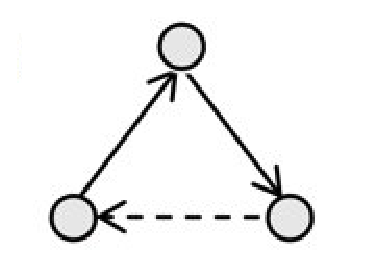
\includegraphics[width=.9\linewidth]{figuras/opfecho_a.eps}
  		\caption{cíclico.}
  		\label{fig:subop1}
	\end{subfigure}%
		\begin{subfigure}{.25\textwidth}
  		\centering
  		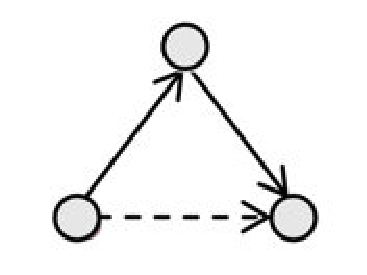
\includegraphics[width=.9\linewidth]{figuras/opfecho_b.eps}
  		\caption{transitivo.}
  		\label{fig:subop2}
	\end{subfigure}%
		\begin{subfigure}{.25\textwidth}
  		\centering
  		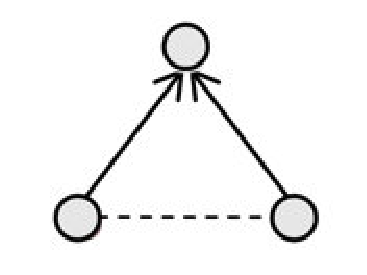
\includegraphics[width=.9\linewidth]{figuras/opfecho_c.eps}
  		\caption{sobrejetor.}
  		\label{fig:subop3}
	\end{subfigure}%
		\begin{subfigure}{.25\textwidth}
  		\centering
  		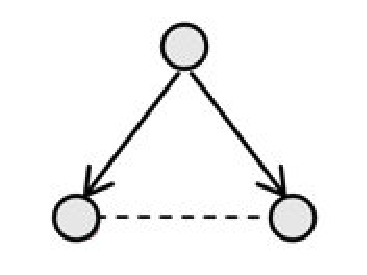
\includegraphics[width=.9\linewidth]{figuras/opfecho_d.eps}
  		\caption{sobrejetor inverso.}
  		\label{fig:subop4}
	\end{subfigure}
	\caption{Operações de fecho.}
	\label{fig:opfecho}
\end{figure}

Com base nessas operações, foram definidos operadores capazes de promover um auto aprendizado da rede. \citeonline{bollen1996} ratificaram essa utilização em uma rede de informações distribuída com múltiplos usuários. Os operadores também foram utilizados em uma rede hipermídia na qual foi incluída a operação de degradação da rede, de modo que os acessos mais recentes tinham maior peso em favor de uma melhor navegação adaptativa \cite{palazzo2000}.

Essas teorias possuem um grande espaço de aplicação em auto organização de sistemas dinâmicos e são utilizadas em diversos campos como cibernética, biologia, termodinâmica, matemática e também evolução da linguagem.

O grande problema dessa abordagem quando aplicada a ambientes de ensino é que não há como relacionar o processo de aprendizagem de um indivíduo ao comportamento comum de usuários em uma rede, pois cada estudante possui objetivos diferentes ou capacidades cognitivas diferentes, dentre várias outras características importantes no processo de ensino e aprendizagem que são únicos para cada pessoa.

A QRN então surge como uma possibilidade de quantização que leve em consideração apenas as informações contidas nos nodos para se gerar a quantização da rede, possibilitando sua utilização em um sistema de cursos on-line \cite{fragelli2010}.

Para se calcular o potencial de ativação entre os nodos da rede é utilizada a menor distância entre o nodo atual e os demais. No caso de uma rede unidimensional de fluxo crescente, se o nodo atual é o nodo cinco e se sua avaliação for satisfatória, o estudante será direcionado para o nodo seis; caso a avaliação seja insatisfatória, o estudante será direcionado para o nodo quatro. Isso exemplifica a utilização da menor distância para se inferir qual o melhor caminho a ser seguido, contudo ainda falta especificar os conceitos, variáveis e condições para se  quantizar a rede, explorados nos tópicos a seguir.

\subsection{Blocos Coesos e Hierarquia de Blocos}

Os blocos coesos são formados por conceitos que não podem ser explicados separadamente, isto é, sempre devem ser apresentados em ordem e não podem ser ocultados individualmente. Por exemplo, a soma de vetores por componentes e a decomposição de vetores são dois conceitos dependentes, pois a decomposição de vetores é necessária para se aprender a soma de vetores por componentes.
Em contrapartida, existem conceitos que abordam um mesmo assunto mas de formas diferentes, que não carecem de uma ordem definida de exibição, como a soma de vetores por componentes e pela regra do paralelogramo. Podem existir inúmeras formas de se explicar um mesmo assunto, por isso é necessário especificar uma hierarquia de blocos, a fim de se especificar um índice de importância para cada uma delas \cite{fragelli2010}.

Essas teorias são de importância maior quando se utiliza um Sistema Tutor Inteligente, pois este atua na seleção de conteúdos para a confecção do material a ser exibido pelo sistema \cite{fragelli2010}, exigindo uma organização dos conceitos dependentes. Já no caso deste trabalho, o material estará pronto a partir do momento que for criado pelo professor autor, não requerendo uma seleção prévia. Entretanto, os blocos coesos podem ser explorados no momento da confecção do material, por meio da criação das ligações entre os nodos, o que dá preferência aos nodos com ligações diretas.

A hierarquia de blocos é também abordada no momento da confecção dos vídeos interativos, mas representa um fator importante para a adaptação da navegação da rede. Uma boa construção de vídeo interativo é necessária para se alcançar bons resultados da adaptação no que diz respeito a seleção de um bloco dentre os existentes na hierarquia.

\subsection{Avaliação e Confiabilidade}

A quantização da rede está diretamente relacionada à avaliação e à confiabilidade dos nodos que a compõem, o cálculo para ambos os valores é feito em duas etapas: direta e indireta. A avaliação direta ocorre quando um estudante responde uma questão do nodo em que se encontra. Isto é, o estudante é avaliado pelo sistema por meio de sua resposta, essa avaliação direta é sucedida pela avaliação indireta do nodo, que corresponde as operações de fecho, e representa os processos de inferência sobre a rede para tentar prever estados futuros. O resultado A da avaliação do nodo é dado pela média ponderada das notas das avaliações direta e indireta, como segue:

\begin{equation}
	A = C_{0}A_{0} + (1 - C_{0})A_{0M}
\end{equation}

Para o cálculo da avaliação indireta, utiliza-se a nota da avaliação do nodo de origem \(A_{1}\) e uma constante \( k_{a},(0 < k_{a} < 5) \), que representa o grau de liberdade para se alterar a nota \(A_{0}\) do nodo. Como na fórmula:

\begin{equation}
	A_{0M} =  A_{0} + (A_{1} - A_{0})\frac{k_{a}}{5}
\end{equation}

O valor da avaliação direta é a média aritmética das notas das questões respondidas do nodo. Por exemplo, se um nodo da rede possui sete questões, o estudante respondeu apenas quatro e tirou nota seis em duas delas e oito nas outras duas, a nota da avaliação direta então será sete. As outras três questões que não foram respondidas não influenciam diretamente o cálculo da avaliação, mas servem para o cálculo da confiabilidade. A avaliação final calculada e finalmente dada por:

\begin{equation}
	 A_{0}=C_{0} A_{0} + (1- C_{0}) \bigg( A_{0}+(A_{1}-A_{0}) \frac{k_{a}}{5} \bigg)
\end{equation}

A confiabilidade \(C_{0}\) do nodo é calculada também por meio de uma média ponderada das duas etapas, direta e indireta. Como mostra a equação:

\begin{equation}
	C_{0}= \frac{(n_a+1) C_0+C_{0M}}{n_a+2}
\end{equation}

Em que \(n_a\) é o número de questões respondidas pelo usuário, \(C_0\) representa a confiabilidade anterior do nodo, \(C_{0M}\) é a confiabilidade da avaliação indireta proposta, que deve aumentar nos casos em que \(A_0\) for um valor próximo de \(A\) e diminuir nos casos em que \(A_0\) e \(A\) forem muito distantes.

\begin{equation}
	\rho_{KR21} = \frac{k}{(k-1)} \bigg(1- \frac{M(k-M)}{ks_{xx}^{2}} \bigg) 
\end{equation}

Na qual, \(k\) é o número de questões, \(M\) é a média dos escores obtidos pelos alunos e \(s_{xx}^{2}\) é a variância corrigida em torno da média, dada por:

\begin{equation}
	s_{xx}^{2} =  \frac{\sum{x^2}}{n-1}
\end{equation}

Em que \(x\) representa a diferença entre o escore do estudante e a média dos estudantes para aquela questão. Nesse sentido, é possível ver que as questões que não foram respondidas terão um valor \(x\) muito alto, o que influencia negativamente no resultado confiabilidade.
	
Da mesma forma, para o cálculo da confiabilidade da avaliação indireta, a distância entre os escores do estudante deve ser levada em consideração, já que, se houver uma variação muito grande entre duas avaliações, isso implica em uma confiabilidade baixa. Além disso, o próprio valor da confiabilidade do nodo de origem influencia o cálculo da nova confiabilidade, como é mostrado abaixo:

\begin{equation}
	C_{0M} = C_1 (1-0,1|A_0 -  A_1 |) 
\end{equation}

Para o cálculo final da confiabilidade, tem-se a seguinte fórmula:

\begin{equation}
	C_0 = \frac{(n_a+1) C_0 + C_1 (1 - 0,1|A_0 - A_1|)}{ n_a+2 }
\end{equation}

\subsection{Influência Temporal}

Para que a rede se adeque aos acessos atuais dos nodos, é realizado um decréscimo percentual da avaliação de um nodo quando um aluno não o acessa durante determinado período de tempo. A ideia é reduzir o grau de interferência das avaliações passadas sobre uma nova retomada do curso, quando o aluno passa algum tempo sem acessá-lo. Esse cálculo é feito da seguinte forma:

\begin{equation}
	A=(1 - p_e)A_0 
\end{equation}

\subsection{Quantização das Ligações entre Nodos}

Como dito antes, a quantização da rede é gerada a partir da menor distância entre os nodos da rede. Esse cálculo é feito levando em consideração o campo tridimensional. Em um primeiro momento, todos os nodos da rede estão em ordem, em \(z=0\) e \(N4\) sendo o nodo atual. O exemplo considera três alterações de nível dos nodos da rede que se referem a blocos coesos, direção e avaliação.

Primeiramente o nodo \(N4\) é colocado em um nível superior da rede de modo que os outros nodos não ultrapassem o nodo atual após as modificações de suas posições (Fig. \ref{fig:subnodos1} ). Posteriormente, todos os nodos que pertencem ao mesmo bloco coeso de \(N4\) sofrem uma elevação de nível (Fig. \ref{fig:subnodos2} ).

\begin{figure}
	\begin{subfigure}{.5\textwidth}
  		\centering
  		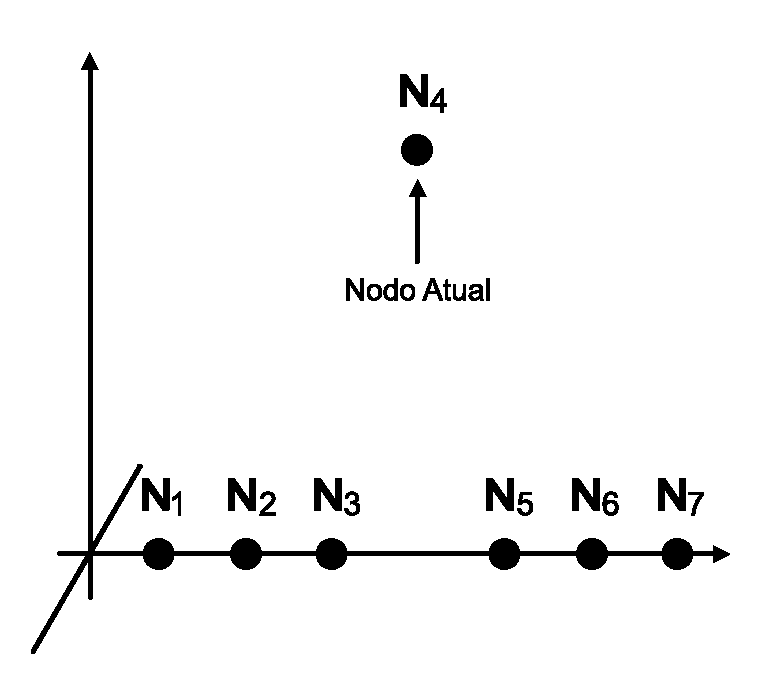
\includegraphics[width=.9\linewidth]{figuras/nodos1.eps}
  		\caption{Deslocamento do nodo atual.}
  		\label{fig:subnodos1}
	\end{subfigure}
	\begin{subfigure}{.5\textwidth}
  		\centering
  		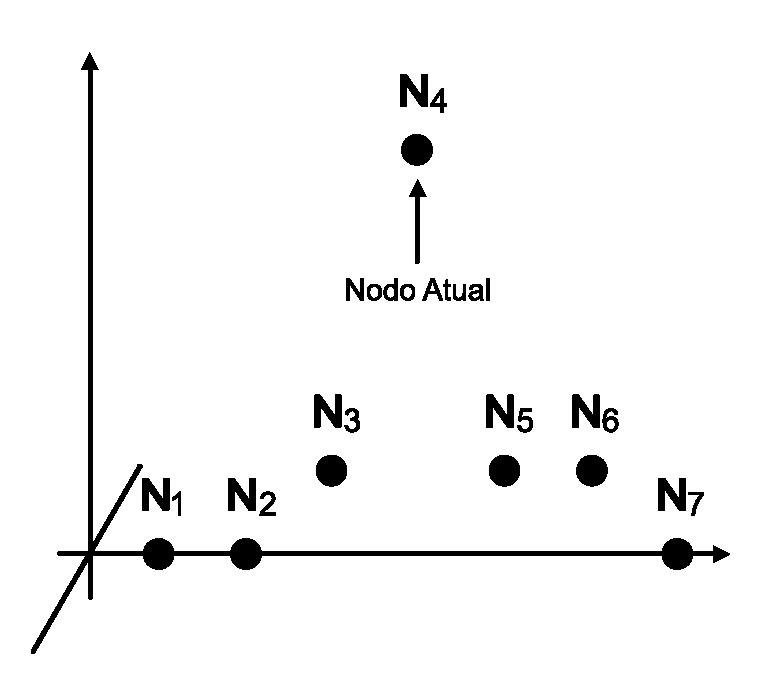
\includegraphics[width=.9\linewidth]{figuras/nodos2.eps}
  		\caption{Deslocamento dos blocos coesos.}
  		\label{fig:subnodos2}
	\end{subfigure}
	\begin{subfigure}{.5\textwidth}
  		\centering
  		\includegraphics[width=.9\linewidth]{figuras/nodos3.eps}
  		\caption{Deslocamento segundo a direção.}
  		\label{fig:subnodos3}
	\end{subfigure}
	\begin{subfigure}{.5\textwidth}
  		\centering
  		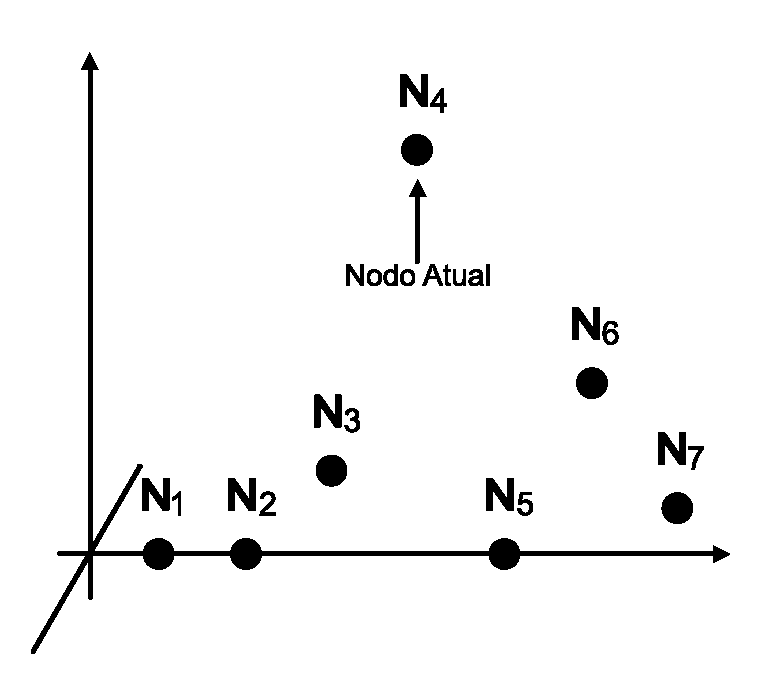
\includegraphics[width=.9\linewidth]{figuras/nodos4.eps}
  		\caption{Deslocamento segunto as avaliações.}
  		\label{fig:subnodos4}
	\end{subfigure}
	\caption{Processo de quantização da rede.}
	\label{fig:nodos}
\end{figure}

Considerando neste exemplo que o estudante tenha obtido um escore superior ou igual ao considerado satisfatório, todos os nodos posteriores ao atual sofrem uma elevação de nível (Fig. \ref{fig:subnodos3}), pois a direção da avaliação indica um avanço positivo. O próximo passo é reduzir proporcionalmente o nível dos nodos com base nas suas respectivas avaliações e confiabilidades (Fig. \ref{fig:subnodos4}).

Com base na nova configuração obtida, basta fazer o cálculo da menor distância entre o nodo atual e os demais para se obter a quantização da rede, segundo a fórmula da menor distância para pontos tridimensionais. Sendo assim, podemos fazer a análise também para a distância ao quadrado, como mostrado:

\begin{equation}
	d^2 = (x_a-x_i)^2 +(y_a-y_i)^2 + (z_a-z_i)^2 
\end{equation}

Essa teoria pode ser utilizada então para redes \(n\)-dimensionais sem prejuízo, pois \(d^2\) é o quadrado da norma euclidiana do vetor distância entre dois nodos da rede \cite{fragelli2010}.

Para que aconteça a quantização da rede, é preciso definir os coeficientes de alteração do nível z e de posicionamento \((x_a,y_a)\) para os nodos, com a finalidade de gerar uma modelagem flexível para diferentes modelos pedagógicos. \citeonline{fragelli2010} ratifica essa afirmação por meio da apresentação de duas propostas de redes quantizadas: behaviorista e cognitivista.

\subsection{Rede Behaviorista Quantizada}

Para uma rede behaviorista, os nodos estão alinhados em x e são dados pelos valores definidos pelo professor ao compor seu curso. Desse modo, a quantização está relacionada à análise de z para o posicionamento dos nodos:

\begin{equation}
	(x,y,z)=(x_a,0,\sum_{i=1}^{m} k_i ) 
\end{equation}

Fragelli propõe a utilização de três coeficientes \(k_i\) para a quantização da rede:

\begin{itemize}
	\item \(k_1\) Blocos Coesos;
 	\item \(k_2\) Direção e Expertise;
 	\item \(k_3\) Avaliação e Confiabilidade.
\end{itemize}

O coeficiente \(k_1\) avalia se um nodo faz parte do mesmo bloco coeso do nodo atual \(N_a\) e define um limite superior de modo que os nodos externos ao bloco coeso não fiquem impedidos de serem acessados.

\[
	(k_1)_i =	\left\{
	\begin{array}{ll}
	    \, p \sum_{j=1}^{k} N_j & \quad \text{ se } N_j \in \text{blocos coesos de } N_a  \\
		\, 0  & \quad \text{ c.c. } \\
  	\end{array}
  	\right.
\]

Nesta equação é possível verificar que \(N_a\) pode pertencer a mais de um bloco coeso e que o coeficiente \(k_1\) do nodo \(N_i\) é o somatório dos elementos dos blocos coesos que contenham \(N_a\) e \(N_i\). Para o escopo deste trabalho, o professor deverá se encarregar de gerar esse coeficiente por meio das distâncias entre os nodos no momento da criação de um curso. Entretanto, este conceito é importante para se entender a possibilidade de adequação da rede para a inserção de um agente pedagógico que possa gerar esses coeficientes analisando a interação do usuário na rede. 

O coeficiente \(p\) está associado ao objetivo do aluno ao acessar um curso, se ele fizer parte do público-alvo para qual o curso foi designado, este aluno poderá seguir o planejamento normal do curso, acessando ordenadamente os nodos.

O coeficiente \(k_2\) é calculado segundo a avaliação do nodo atual \(N_a\) e o fluxo normal indicado pelo autor. Para um nodo \(N_i\), o valor de \(k_2\) é dado por:

\[
	(k_2)_i =	\left\{
	\begin{array}{ll}
	    \, v 	& \quad \text{ se }  A_{N_a} \ge  p_b\varepsilon_{N_a}  \text{ e } x_{N_j} > x_{N_a}  \\
	    \, v 	& \quad \text{ se }  A_{N_a} < p_b\varepsilon_{N_a}  \text{ e } x_{N_j} < x_{N_a}  \\
	    	\, 0  	& \quad \text{ c.c. } \\
  	\end{array}
  	\right.
\]

Para determinação do valor de v, deve-se verificar o valor necessário para provocar uma tendência de seguir o fluxo normal do curso, para isso é necessário treinar a rede, semelhante ao processo de treinamento das redes neurais. O coeficiente \(p_b\) indica qual o percentual da expertise \(\varepsilon_{N_a}\) seria suficiente para uma avaliação satisfatória do nodo.

O coeficiente \(k_3\) tem o objetivo de diminuir a chance de um nodo com avaliação satisfatória e confiabilidade alta ser acessado. Sendo assim, este coeficiente é dependente dos valores de \(k_1\) e \(k_2\) calculados anteriormente. A solução proposta por Fragelli envolve a relação linear:


\[
	(k_3)_i = - \min \Bigg(  \frac{\min( \frac{C_{N_j}}{C_0} , 1)A_{N_j}}{p_b\varepsilon_{N_j}} , 1  \Bigg)(k_1 + k_2)
\]

Desse modo, se um nodo possui avaliação satisfatória e confiabilidade superior à confiabilidade mínima \(C_0\) o valor de \(k_3\) será \(-(k_1+k_2)\) e o nodo retornará para \(z=0\). Em qualquer outra situação, a redução será proporcional aos valores da avaliação e da confiabilidade do nodo \(N_j\).

\subsection{Rede Ausubeliana Quantizada}

No caso de uma rede levando em consideração a teoria de Ausubel, são utilizados os mesmos coeficientes de nível da rede behaviorista, com uma modificação que é a utilização das posições dos nodos no mapa conceitual construído pelo professor. Assim, a distribuição espacial dos nodos no momento da construção do curso é bastante útil na quantização da rede que ficaria:

\begin{equation}
	(x,y,z)=(x_a,y_a,\sum_{i=1}^{m} k_i ) 
\end{equation}

Onde \((x_a,y_a)\) representam a posição do nodo no mapa conceitual da rede. O grande avanço desta proposta é a possibilidade da modificação do mapa conceitual para cada estudante distinto que acessa a rede, suas características influenciam também a disposição dos elementos. Uma grande discussão sobre o uso dos mapas conceituais é que o mapa conceitual construído pelo professor nem sempre representa o mapa que seria feito pela estrutura cognitiva do estudante, por isso é importante o desenvolvimento de um sistema que permita a adaptação do mapa conceitual segundo as impressões do estudante.

Com base no aporte teórico educacional apresentado, é necessário compreender também os métodos e técnicas do estudo em engenharia de software que proporcionem meios suficientes para que o sistema proposto possa ser desenvolvido, sendo estes apresentados a seguir.

\section{Arquitetura de software}

Ao passo que os sistemas de software se desenvolvem em tamanho e complexidade, os problemas de projeto vão além dos algoritmos e estruturas de dados: projetar e especificar a organização geral do software surge como um novo problema. Falhas estruturais incluindo mecanismo global de controle; protocolos de comunicação, sincronização e acesso de dados; distribuição física; composição dos elementos do projeto; escalabilidade e performance; e seleção dentre as alternativas de design. Esse é o nível arquitetural do projeto de software \cite{shaw1996}. 

Este nível de projeto de software possui um grande conjunto de trabalho, decisões sobre padrões de projeto, utilização de paradigmas, \textit{frameworks} e modelos arquiteturais que são de suma importância para redução de retrabalhos e aumento da qualidade e manutenabilidade do produto final \cite{krasner1988}.

O modelo arquitetural MVC (do inglês \textit{Model - View - Controller}) é um estilo fundamentado no modelo de arquitetura em camadas, primeiramente idealizado por \citeonline{reenskaug1979} em 1978 para um projeto específico chamado \textit{Smalltalk}. Tendo como objetivo separar o modelo de negócio abordado no sistema (camada \textit{Model}), da camada de interface com o usuário (\textit{View}), permitindo que esse modelo possa ser exibido de inúmeras e diferentes formas sem ter conhecimento de quem o está exibindo \cite{krasner1988}. A fig. \ref{fig:krasner} ilustra o funcionamento da arquitetura MVC e as interfaces entre camadas. 


\begin{figure}[h!]
	\centering
  	\includegraphics[width=.9\linewidth]{figuras/mvc.eps}
  	\caption{Model - View - Controller.}
	\small{Fonte: \cite{krasner1988}}
  	\label{fig:krasner}
\end{figure} 

Para manter todas as \textit{Views} e \textit{Controllers} atualizadas segundo o estado da \textit{Model}, foi definida também a noção de dependência. Os objetos do tipo \textit{Controller} e \textit{View} são registrados em uma lista de dependentes na \textit{Model}, e quando ocorre alguma mudança no estado do modelo, estes são avisados através de troca de mensagens \cite{krasner1988}. 

Anos depois, no final da década de 1980, o paradigma foi publicado como um padrão arquitetural para sistemas \textit{web}, no sentido de que é interessante que o modelo não conheça a forma de apresentação, já que uma página pode ser exibida em diferentes dispositivos com diferentes resoluções e proporções de tela, e que deve se comportar de forma diferente sem comprometer o bom funcionamento do sistema \cite{krasner1988}. Se tornando uma forte tendência para estas aplicações desde então.

Esta estrutura arquitetural foi utilizada inicialmente para renderização \textit{server-side} \cite{shabaitah2014}, ou seja, o processo digital sobre a página é feito no servidor que provê o serviço \textit{web}, sendo esta necessária, já que no início da década de 90, poucos computadores pessoais possuiam capacidade para executar o processamento das páginas depois de recebidas e que ainda hoje existem dispositivos com pouca capacidade de processamento que também fazem consultas a internet e dependem do servidor para renderização, como equipamentos de e-books e alguns smartphones\cite{baker2006}. 

Com o desenvolvimento de navegadores mais robustos e com funcionalidades diversas, construir aplicações que dependem de renderização no cliente se tornou não somente factivel, mas bastante popular \cite{google2015}. Nesse sentido o estilo arquitetural MVC para aplicações \textit{web} tem sofrido consideráveis mudanças, de modo que camadas da aplicação antes existentes apenas nos servidores passaram a executar papéis importantes também no cliente \cite{google2015}.

\begin{figure}[h!]
	\centering
  	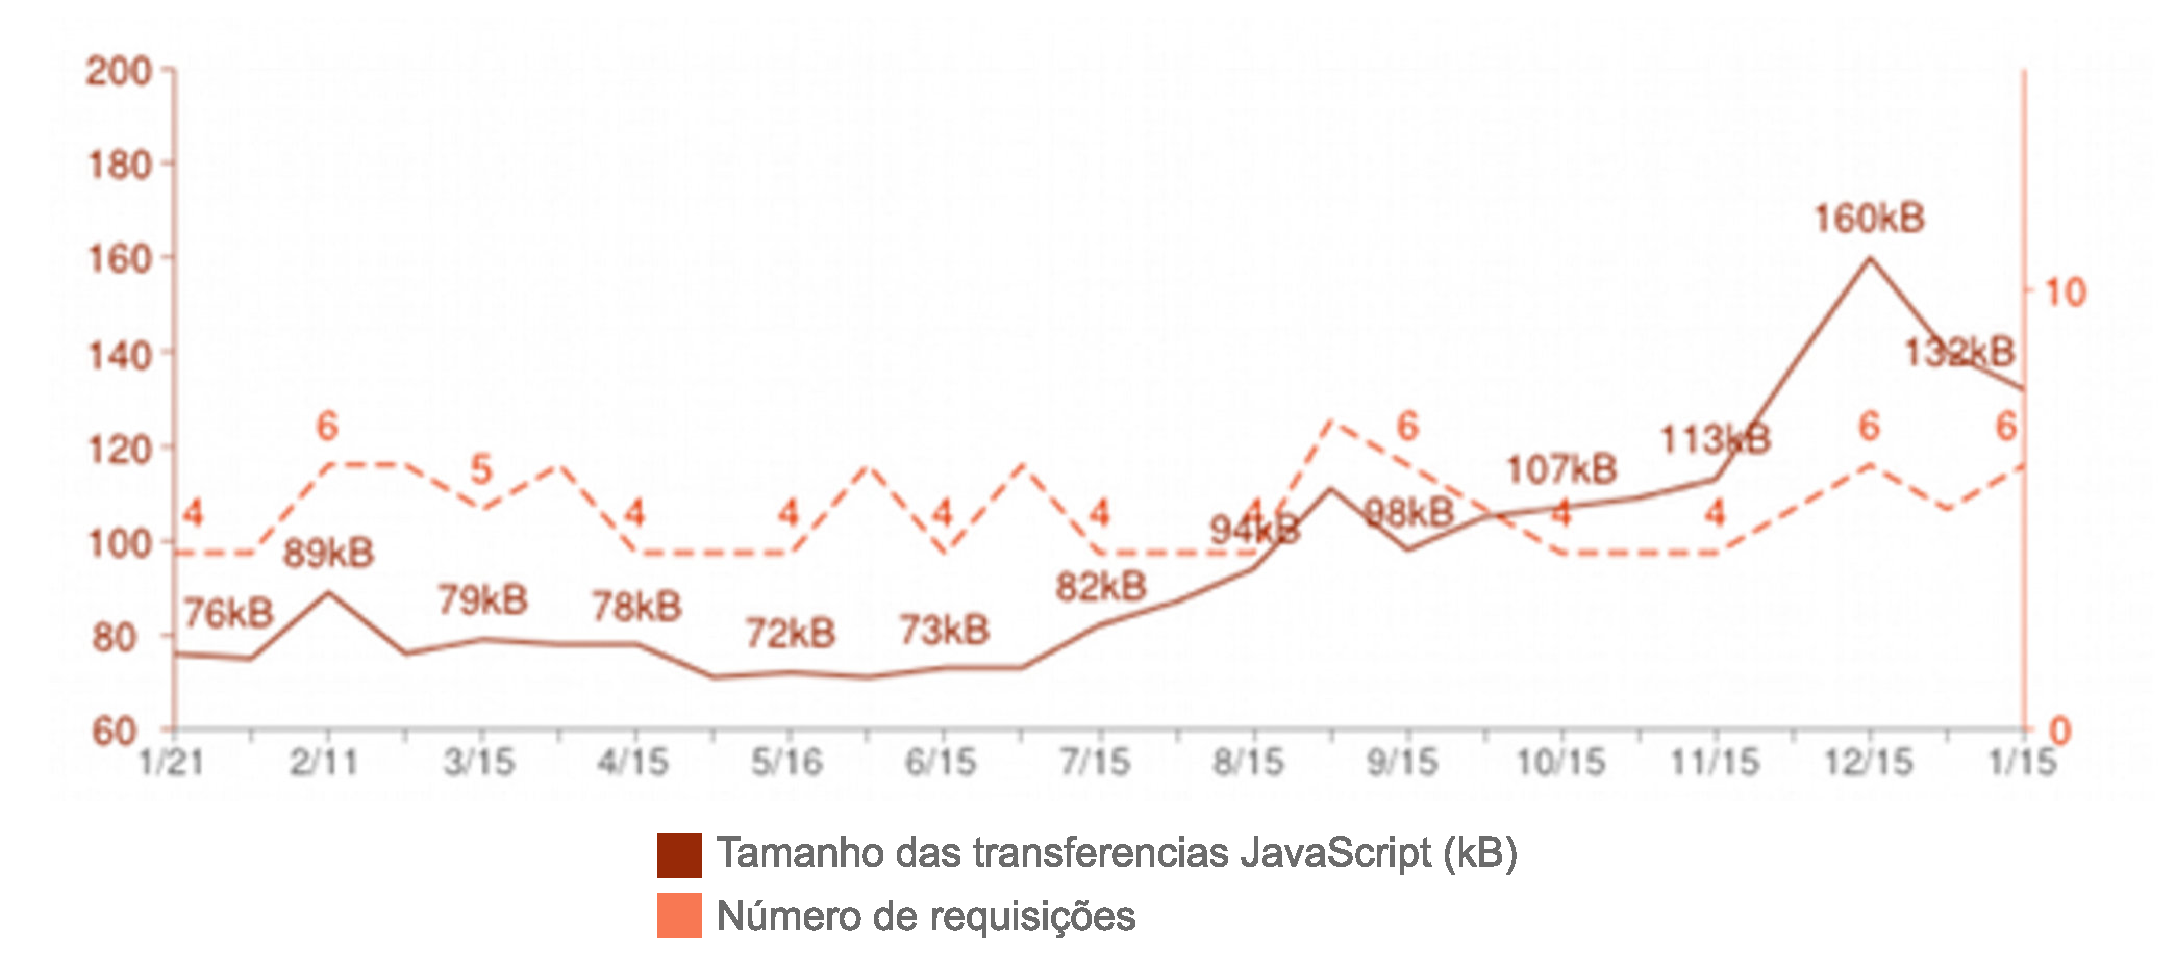
\includegraphics[width=.9\linewidth]{figuras/jsdata.eps}
  	\caption{transferências e requisições JavaScript.}
	\small{Fonte: \cite{google2015}}
  	\label{fig:jsdata}
\end{figure}

A figura \ref{fig:jsdata} mostra o crescimento da popularidade de arquivos \textit{JavaScript} em páginas \textit{web}, linguagem mais comumente usada para aplicações que são executadas no lado do cliente e que podem também gerenciar renderização. 

Com base no que foi apresentado, é possível encontrar na literatura várias formas de implementar uma arquitetura MVC com renderização no servidor, no cliente ou em ambos. A figura \ref{fig:mvc} a seguir ilustra alguns exemplos genéricos encontrados em ferramentas bastante utilizadas atualmente \cite{mejia2011, petitit2014, quinn2015}. 

Uma arquitetura \textit{web} tradicional, utiliza em geral renderização no servidor e retorna a página pronta para o cliente que interage por meio de controles providos pelo navegador, redirecionando as requisições ao servidor, que executa o processamento e retorna uma nova página ao cliete após a resposta à requisição ser construída. Para essa estrutura, a cada ação do usuário, uma nova requisição é criada e existe uma latência considerável entre executar a requisição e receber a resposta novamente no cliente \cite{mejia2011}.

Para uma arquitetura no cliente ou uma arquitetura mista, existem \textit{frameworks} que provêm recursos suficientes para persistencia e controle no cliente. No caso da arquitetura mista, podem existir APIs no servidor implementados em diversas linguagens para gerenciar requisições e envios de dados ao cliente, além da possibiliade de responderem uma página renderizada \cite{ petitit2014, quinn2015}. Já para aplicações que possuem um MVC completo no cliente, o servidor pode servir meramente como um banco de dados, que provê as informações necessárias ao cliente por meio de uma API publish subscribe \cite{quinn2015}.

\begin{figure}[h!]
	\centering
	\begin{subfigure}{.31\textwidth}
  		\centering
  		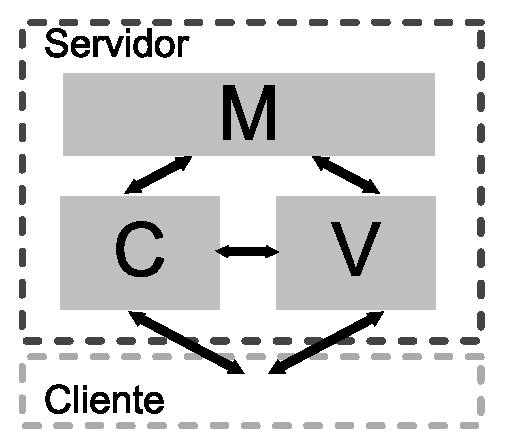
\includegraphics[width=.9\linewidth]{figuras/servidor.eps}
  		\caption{\textit{server-side}.}
  		\label{fig:submvc1}
	\end{subfigure}
	\begin{subfigure}{.31\textwidth}
  		\centering
  		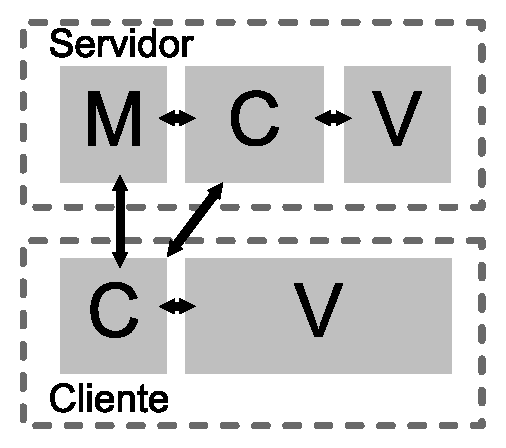
\includegraphics[width=.9\linewidth]{figuras/misto.eps}
  		\caption{misto.}
  		\label{fig:submvc2}
	\end{subfigure}
	\begin{subfigure}{.31\textwidth}
  		\centering
  		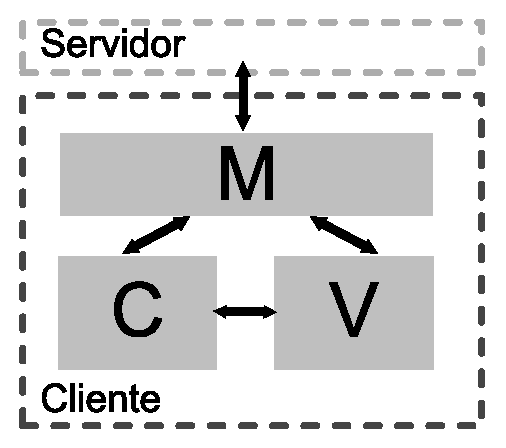
\includegraphics[width=.9\linewidth]{figuras/cliente.eps}
  		\caption{ \textit{client-side}.}
  		\label{fig:submvc3}
	\end{subfigure}
	\caption{Estilos Aquiteturais MVC.}
	\label{fig:mvc}
\end{figure}

Apesar de suas diferenças e semelhanças, cada modelo possui vantagens e desvantagens. No caso de renderização no servidor, uma grande vantagem é a independência do cliente, que caso possua pouca capacidade de processamento, conseguirá executar a aplicação sem grandes problemas. Já para aplicações com renderização no cliente, é necessário que o dispositivo seja veloz o suficiente para executar a aplicação. Apesar disso, aplicações com renderização no cliente possuem geralmente uma interface mais rica e usável \cite{Ubl2015}. No caso deste trabalho, é proposta uma arquitetura mista, detalhada no capítulo 3 sobre o desenvolvimento.

Independente de onde aconteça a renderização, o MVC possui vantagens como possibilidade de reuso de código, separação entre níveis conseituais e menor acoplamento entre as camadas, possibilitando maior manutenabilidade e qualidade do código produzido \cite{krasner1988}. Entretanto, a qualidade do \textit{software} não é medida unicamente por sua arquitetura, testes são meios menos abstratos de se garantir a qualidade do software desenvolvido. A seguir, descorre-se sobre estratégias e tipos de testes encontrados na literatura.

\section{Testes de Software}

O processo de teste de software procura determinar se um sistema atinge suas especificações e funciona corretamente no ambiente para o qual foi projetado, tendo como objetivo identificar falhas durante o desenvolvimento para que possam ser corrigidas antes da entrega do produto final  \cite{neto2005}. 

Para entender o conceito de testes, é necessário compreender a diferença entre defeito, erro e falha. Um defeito se encontra no meio físico, é uma instrução de um passo, ou deifinição de dados incorreta. Um erro está no âmbito da informação, na construção de um software diferente do que foi especificado, sendo qualquer passo intermediário diferente do que é esperado. Uma falha, por sua vez, é o comportamento inesperado que afeta diretamente o usuário final da aplicação, podendo inviabilizar o uso do sistema \cite{ieee1990}, como ilustra a figura \ref{fig:erro}. 

\begin{figure}[h!]
	\centering
  	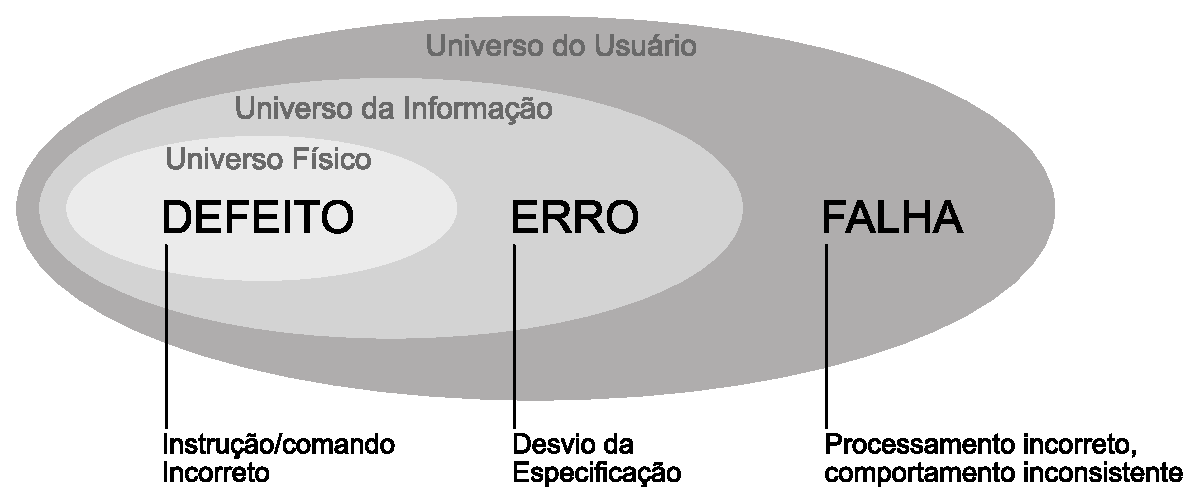
\includegraphics[width=.9\linewidth]{figuras/erro.eps}
  	\caption{Defeito \(\times\) Erro \(\times\) Falha.}
  	\label{fig:erro}
\end{figure}

Testes podem ser projetados de dois pontos de vista: estrutural ou funcional. Os testes funcionais ignoram o mecanismo interno de execução e se concentram nos resultados gerados com o propósito de encontrar não conformidades com a especificação da funcionalidade. Testes funcionais são direcionados ao usuário e devem se preocupar unicamente com a funcionalidade. Já os testes estruturais analisam o funcionamento interno em diferentes níveis, podendo envolver todo o sistema, ou apenas partes dele. Para \citeonline{naik2008}, existem 3 níveis de testes estruturais, sendo eles de unidade, integração e sistema.

Testes unitários são utilizados para testar de forma isolada funções, métodos ou classes. Após garantir que as unidades funcionam de forma satisfatória, os módulos são agrupados para se construir sub-sistemas maiores que são testados por meio das técnicas de teste de integração. Testes unitários são importantes pois, uma vez que o código está integrado a outros módulos, encontrar a causa de uma falha, se torna mais difícil \cite{naik2008}. Existem diferentes ferramentas de teste unitário para diversas linguagens, porém a maioria provê recursos semelhantes para construção de acertivas afim de verificar se os resultados retornados pelo código testado está de acordo com a especificação proposta, algumas dessas ferramentas são JUnit \cite{junit2015}, ActiveSupport \cite{activetest2015}, Mocha \cite{mocha2015}.

As ferramentas citadas acima podem ser utilizadas também para construção de testes de integração. Testes estes que são efetuados de modo incremental, adicionando e testando, a cada ciclo, um novo módulo do sistema. Esse processo é repetido até que todos os módulos tenham sido integrados e testados. Esse nível de teste examina explicitamente as interfaces entre unidades a fim de verificar se o sistema é capaz de suportar testes do nível de sistema \cite{naik2008}.

Os testes a nível de sistema englobam testes básicos de instalação e configuração; testes funcionais estensivos sobre todo o sistema; testes de robustez para verificar quão bem o sistema se recupera de situações de falha; testes de interoperabilidade, performance e escalabilidade e também testes de stress, para verificar os limites do sistema e em quais situações a falha ocorre. Muitos dos testes de sistema dependem diretamente do ambiente no qual o software será instalado e utilizado, pois necessitam aproximar os resultados para um ambiente o mais próximo do real possível \cite{naik2008}.


\section{Metodologia \textit{Scrum}}

O \textit{Scrum} é um framework ágil para gerenciamento de projetos, fundamentado no empirismo. O empirismo afirma que o conhecimento provém da experiência e de tomadas de decisões baseadas no que é conhecido. Desse modo, o \textit{Scrum} utiliza do método da inspeção e adaptação para reagir a mudanças e melhor lidar com a complexidade e riscos do projeto. Outro aspecto importante do método é o foco no aprendizado e difusão do conhecimento, em que todos os integrantes do time cooperam para o aprendizado coletivo e para um melhor desenvolvimento do produto \cite{scrum2013}. 

O \textit{Scrum} pode ser utilizado em diferentes contextos. Entretanto, surgiu para suprir uma demanda clara do processo produtivo da indústria de software, na qual inúmeros projetos falharam pela ineficiência dos processos produtivos em cascata, mais utilizados até meados dos anos 90, em projetos que custaram milhões e resultaram em fracaço para grandes organizações como \textit{FBI (Federal Bureau of Investigation)} ou \textit{NPR (National Public Radio)} \cite{scrum2014}.

Para este trabalho, foram levados em consideração quatro princípios básicos da metodologia listados por \citeonline{scrum2014}, sendo eles: 
	\begin{itemize}
		\item \textbf{Planejar é útil. Seguir cegamente os planos é burrice.} Simplifique o processo de planejamento e aja o quanto antes. Reavalie o seu planejamento com frequência, especular sobre o desconhecido é pouco eficaz, devido à dificuldade de se controlar inúmeras variáveis do processo.
		\item \textbf{Inspeção e Adaptação.} De tempos em tempos é necessário rever o trabalho que foi desenvolvido e verificar se o caminho traçado ainda está correto, ou se existem formas melhores de fazê-lo.
		\item \textbf{Mudar ou Morrer.} Ficar preso em métodos antigos de mandar e controlar ou manter uma previsibilidade rígida resultará no fracasso. A mudança gera vantagens estratégicas e comerciais e deve sempre ser bem-vinda.
		\item \textbf{Fracasse rápido para corrigir o problema o quanto antes.} Todo o trabalho que gera um desperdício de esforço deve ser eliminado, possibilitando que produto real seja entregue ao usuário com o tempo e esforço economizados.
	\end{itemize}
	
Claramente, os termos utilizados pelo autor são metafóricos, mas indicam de forma simples a ideia por trás dos tópicos.

Por fim, uma ultima prática que necessita de destaque para qualquer desenvolvimento ágil de software,  é o processo de integração contínua. Os times que utilizam essa prática visam alcançar dois resultados primários: a redução do custo para se requerido para cada episódio de integração dos componentes do sistema e a possibilidade de entrega de produto funcional a qualquer momento do desenvolvimento \cite{agile2015}.

Na prática, estes objetivos requerem um processo de integração que seja passível de reprodução, pelo menos, em sua grande maioria, e que seja "automático". Isto é conseguido através de ferramentas de controle de versão, políticas e convenções da equipe e ferramentas projetadas especificamente para ajudar a alcançar a integração contínua \cite{agile2015}.

